\documentclass[11pt]{article}
\usepackage[margin = 1in]{geometry}
\usepackage{amsmath}
\usepackage{amssymb}
\usepackage{amsthm} % for proof environment
\usepackage{enumitem}
\usepackage{graphicx}
\usepackage{indentfirst}
\usepackage{caption}
\usepackage{lscape}
\usepackage{multirow}
\usepackage{array}
\usepackage{setspace}
\setlist{nolistsep}
\usepackage[round]{natbib}
\usepackage{accents}
\usepackage{caption}
\usepackage{subcaption}
\usepackage{xcolor}
\usepackage{setspace}
\onehalfspacing

\newcommand{\ubar}[1]{\underaccent{\bar}{#1}}
\newcommand{\p}{\prime}
\newcommand{\ev}{\mathbb{E}}
\newcommand{\lagr}{\mathcal{L}}
\newcommand{\inv}[1]{#1^{-1}}
\newcommand{\R}{{\rm I\!R}}
\newcommand{\U}{\mathcal{U}}
\renewcommand{\H}{\mathcal{H}}
\newcommand{\pderiv}[2]{\frac{\partial#1}{\partial #2}}
\newtheorem{proposition}{Proposition}
\newtheorem{lemma}{Lemma}

% Front matter
\title{Optimal Taxation with Heterogeneous Rates of Return}
\author{
    Nicholas Hoffman\\
    \and 
    Ali Shourideh\\
}
\date{\today}

\begin{document}
\maketitle
\begin{abstract}
    We study optimal capital taxation in a model in which individuals are heterogeneous in the rates of return that they face. By offering individuals the choice between risk-free saving and risky investing, we capture the role that the government plays in ensuring that its most able entrepreneurs invest capital into their businesses. We allow the government to levy separate taxes on interest income from risk-free savings and on capital income earned by investing into private entrepreneurial enterprises. We begin in a static, two-period setting, and demonstrate properties of constrained-efficient allocations both analytically, and in a numerical model. We then turn to a fully dynamic model, and demonstrate that the optimal allocations and wedges in this setting are independent of an agent's history of capital income. Finally, we discuss the implementation of these allocations in a decentralized economy with taxes and transfers. 
\end{abstract}

\section{Introduction} \label{sec:intro}

Recent advances in data collection and economic modelling have given economists a strong understanding of the way in which the distribution of wealth in the United States has evolved to its current shape.\footnote{See for instance \cite{benhabib2011distribution} or \cite{benhabib2019wealth}.} We know that the fortunes of those on the top rung of the economic ladder are primarily composed of risky assets such as ownership of businesses and shares of stock. These fortunes are held by entrepreneurs, investors, and business owners---talented individuals who face a range of risks and rates of return in accumulating their wealth. Given these forces shaping the wealth distribution, however, it is less clear what sort of tax and transfer system is optimal to both satisfy the redistributive motives of the government and encourage investors to undertake risky projects with benefits that are beneficial to society. In order to study this question, we construct a model in which agents face differing rates of return, and a benevolent government levies taxes in order to satisfy utilitarian redistributive motives. 

The best way in which to tax the wealthy is a central focus of the current political debate. \cite{saez2019triumph} argue that, if one accounts for state, local, and sales taxes, the richest one hundredth of Americans pay a disproportionately small share of their income in taxes. Saez and Zucman attribute this regressive feature of the ex-post tax system to the treatment of capital income: owners of capital, they argue, are able to control the timing, amount, and even location of their income in a way that laborers are not. As a solution, they propose a tax on wealth directly, which they argue is more difficult to move or conceal. Critics of this approach note that such a tax discourages the type of risky investment that has long been the engine of economic growth. 

The Dynamic Public Finance literature, which began with the seminal work of \cite{mirrlees1971exploration}, offers us a way in which to weigh these concerns in implementing optimal capital taxation. What distinguishes this literature from prior work in optimal taxation (``Ramsey'' taxation) is that no exogenous restrictions are imposed on the tax schedule. Instead, the government can implement any type of tax that it wishes, subject to revenue requirements and endogenous informational frictions. Given the nonlinear tax schedules and informational frictions present in reality, we view this as an intuitively appealing setting in which to study capital taxation. 

A canonical result in the Ramsey literature, in which the government seeks to raise its revenue using the most non-distortionary linear taxes possible, is that the tax on capital should be set to zero.\footnote{See for instance \cite{atkinson1976design}, \cite{chamley1986optimal}, and \cite{judd1982redistributive}.} Perhaps the simplest reasoning behind this result is that the supply of capital is highly elastic, and any distortions introduced to the savings decisions of agents in the economy will decrease the future capital stock. In the presence of informational frictions, by contrast, it is often the case that capital taxes are nonnegative at the optimum.\footnote{\cite{golosov2003optimal} show this result in a general setting.} In this case, the government taxes capital in order to prevent agents from self-insuring against idiosyncratic income shocks, ensuring that they will continue to exert labor effort. In most cases, however, these results arise in environments wherein even the wealthiest agents earn the bulk of their income in the labor market, and everyone saves at a common, risk-free rate. We investigate whether the optimality of nonnegative intertemoporal wedges remains when individuals face risk to their rates of return, and when the primary way in which wealthy agents earn income is through returns to capital--as is the case in reality. 

Given these wedges, we then turn to implementation in a competitive, dynamic economy. Studying implementations provides further motivation for allowing rates of return to be heterogeneous across the population. If all assets earn a constant rate, then there is an equivalence between taxing wealth and taxing capital income, and to a certain extent, either can be used to appropriately discourage savings. With different rates of return, however, this equivalence is lost, and taxes on capital income and wealth have fundamentally different impacts on behavior, and consequently, on government revenues. For this reason, a setting with heterogeneous and stochastic rates of return is an appropriate context for studying the different impacts of these tax schemes. 

We also consider this work a step in studying optimal taxation in the face of plausible processes for wealth accumulation. A number of different augmentations have been introduced to the workhorse heterogeneous models of \cite{aiyagari1994uninsured} and \cite{huggett1996wealth} in order to generate long-run distributions of wealth that match their empirical counterparts. Examples of such augmentations include \cite{quadrini2000entrepreneurship}, \cite{hubmer2016historical}, and \cite{benhabib2019wealth}, all of which produce long-run distributions of wealth more in line with the data. The widespread use of augmentations such as these demands a more thorough understanding of optimal taxation in a setting where agents face differing returns to saving. Our goal is to begin to build such an understanding: though at times we refer to agents who save capital in risky vehicles as ``entrepreneurs,'' our results apply to any setting in which agents can choose a portfolio of investments of varying risk and return. 

We proceed as follows. Section \ref{sec:lit_rev} reviews the progress made in the literature around this topic to date, and highlights precisely how we aim to expand on these findings. In section \ref{sec:two_pd}, we present a two-period version of our model, in which we establish results on optimal intertemporal (savings) wedges. In section \ref{sec:dyn_mod} we to the fully dynamic model. Here, we demonstrate that optimal wedges are independent of history, and discuss how the constrained-efficient allocations might be implemented in a decentralized market economy. Section \ref{sec:conc} concludes. 

\section{Literature Review} \label{sec:lit_rev}

Our study builds primarily upon a long line of research on optimal taxation. \cite{mirrlees1971exploration} introduced the canonical model, a static economy in which agents are privately informed of their own ability to turn labor effort into output. In contrast to prior literature, Mirrlees allowed the government to choose nonlinear tax schedules, provided that they incentivized each type to exert its allocated effort. Nevertheless, in his numerical examples, he found that the optimal labor income tax schedule was approximately linear over most of the distribution of productivities, and zero at the top and bottom. Following \cite{mirrlees1971exploration}, \cite{diamond1998optimal} and \cite{saez2001using} demonstrated, using empirically plausible preferences and distributions of ability, that while the optimal tax schedule may in fact be quite nonlinear, it is increasing in income, or progressive, over most of the distribution of ability.

\cite{golosov2003optimal}, \cite{kocherlakota2005zero}, and \cite{albanesi2006dynamic} extend this approach to dynamic economies, in which agents' skills evolve stochastically over time and risk-free savings is the only vehicle for self-insurance. \cite{golosov2003optimal} derive one of the key results in this literature: they demonstrate that for a wide class of specifications for the risk that agents face, the optimal tax system distorts their intertemporal consumption-savings decision, discouraging them from carrying too many assets into each period. \cite{kocherlakota2005zero} shows that this result holds in an economy subject to aggregate shocks. He also shows that the intertemporal wedge can be implemented by a tax system that is nonlinear in capital gains and linear in current wealth, and that in such a system, the tax on wealth is zero in the aggregate and raises no revenue. \cite{albanesi2006dynamic} construct a dynamic economy in which agents are subject to idiosyncratic shocks to their disutility of labor, and show that optimal allocations can be implemented in a market economy using a simple tax schedule conditioned on wealth and current labor income. In this decentralization, the tax on capital may be nonzero, depending on how the tax system incorporates an agent's labor income history. 

One common feature of these three papers is that the intertemporal rate of return on savings is constant across individuals, even if it may vary over time. Such a process of accumulation, however, fails to capture the way in which wealth is built in reality. \cite{benhabib2011distribution} show that the main force behind the thick tails in the wealth distribution-- such as those in the US data--is variation in individual rates of return. To see intuitively why this is the case, consider two favorable shocks to an agent: one affects his income, and the other affects the rate of return. The shock to income allows him to save more, increasing his wealth additively. The shock to his rate of return, however, \textit{multiplies} his wealth. It is this second type of shock that fills in the thick upper tail in the stationary distribution of wealth--particularly if an agent has the potential to realize several such favorable shocks consecutively.

Because variable rates of return can help models capture the thick tail in the empirical wealth distribution, a more recent strand of literature has attempted to characterize optimal taxation in settings where agents earn heterogeneous returns. \cite{phelan2019differential} considers a framework in which agents can hold a number of different assets, and the government is able to tax income from these assets according to different schedules. He finds that the tax on income from risky capital is constant throughout the population, and dependent only on the degree to which information is private, rather than individual productivities. In our model, the optimal tax on risky investment income does depend on the individual's idiosyncratic rate of return, or type. \cite{phelan2019business}, meanwhile, studies optimal wealth, labor, and capital income taxation in a context similar to ours, in which business owners' returns evolve according to a law of motion that depends upon their history of effort, as well as a random drift. Where our approaches differ is in the forces that generate disparate returns: agents in \cite{phelan2019business} have utility over consumption and leisure, and earn higher returns by investing more \textit{effort} over time. Our model, meanwhile, abstracts away from this mechanism, instead treating agent's average returns as an intrinsic characteristic, and allocating to entrepreneurs the investment of capital rather than effort.   

Our model is most closely related to that in \cite{shourideh2014optimal}, in which agents are subject to both ex-ante and ex-post heterogeneity in the returns to their entrepreneurial investments. In this environment, where type, investment, and ex-post shocks are all unobservable, the optimal wedges for both risky investment and risk-free savings are increasing in type \( \theta \). We build upon this work in two ways. To begin, we reduce the ex-post heterogeneity in returns to two states, rather than a continuum. This change both makes the model more tractable, and allows us to consider a distribution for type \( \theta \) that is unbounded. In addition, we explicitly compare implementing the tax system with wealth and capital income taxes separately, and in doing so, aim to shed light on whether a tax on capital ought to depend on an agent's entire accumulated stock of assets, or just his most recent realized return. 

\section{Two-Period Economy} \label{sec:two_pd}

Our model is most closely related to that in \cite{shourideh2014optimal}. Although the full model is of infinite length, for expositional purposes, we begin with a two-period version of the model, in which a number of results on optimal taxation in the full model can be shown. 

\subsection{Model} \label{sec:two_pd_model}

The economy is populated by a continuum of agents, indexed by \( i\in[0,1] \). Each agent has a privately-known type \( \theta\in\Theta=[\ubar{\theta},\bar{\theta}] \), distributed according to the C.D.F \( F(\theta) \). Time is discrete, and is given by \( t\in\{0,1\} \). Agents derive utility from consumption and discount the future at rate \( \beta \). All agents are endowed with initial wealth \( w \), which they allocate at \( t = 0 \) between consumption and savings. There are two assets in which agents may save for future consumption: risk-free savings bonds \( b \), and investment into their private entrepreneurial production technology \( k \). The price of the risk-free bond is normalized to one, and its return given by \( R > 0 \). If an agent of type \( \theta \) invests \( k \) into his entrepreneurial technology, his production at \( t = 1 \) is as follows:
\begin{equation}
    y = \begin{cases}
        \theta k & \text{with probability }\alpha \\
        0 & \text{with probability }1 - \alpha
    \end{cases}
\end{equation}
where \( \alpha \) is an exogenous parameter. 

The government levies a tax on capital income, and is able to differentiate between income from risk-free saving and risky investment. Thus, the tax function has the form \( T(y,Rb) \), and the partial derivatives \( T_1 \) and \( T_2 \) give the marginal tax rates on the two types of investment income. The government is unable, however, to observe type \( \theta \), investment \( k \), or shock \( \varepsilon \). As noted in \cite{mirrlees1971exploration}, the government can be equivalently characterized as a benevolent social planner, who collects reports from agents on their type \( \theta \) and income \( y \), and allocates first-period consumption and investment \( \left( c_0(\theta),k(\theta) \right) \) and second-period consumption \( c_1(\theta,y) \) and \( c_1(\theta,0) \) upon realization of a successful and unsuccessful investment, respectively. Henceforth, we use the terms ``government'' and ``planner'' interchangeably. 

The planner's objective, then, is to maximize
\begin{equation}
    \int_{\ubar{\theta}}^{\bar{\theta}}\U(\theta)f(\theta)d\theta \label{eqn:plan_obj}
\end{equation}
where 
\begin{equation}
    \U(\theta) = u\left(c_{0}\left(\theta\right)\right)+\beta\left[\alpha u\left(c_{1}\left(\theta,y\right)\right)+\left(1-\alpha\right)u\left(c_{1}\left(\theta,0\right)\right)\right]) \label{eqn:pkc}
\end{equation}
by choosing allocations \( \left( c_0(\theta),k(\theta) ,c_1(\theta,y) \right)\) for \( \theta\in\Theta \) and \( y\in\R_+ \). Throughout this paper, we assume that \( u(c) = \log(c) \). An allocation is said to be \textit{feasible} if it satisfies the resource constraints for \( t=0,1 \):
\begin{align}
    \int\left[c_{0}\left(\theta\right)+k\left(\theta\right)\right]dF\left(\theta\right)&\le w \label{eqn:rc0} \\
    \int\left[\alpha c_{1}\left(\theta,y\right)+\left(1-\alpha\right)c_{1}\left(\theta,0\right)\right]dF\left(\theta\right) &\le \int\alpha\theta k\left(\theta\right)dF\left(\theta\right) \label{eqn:rc1}
\end{align}

Additionally, because the planner cannot observe \( \theta \) or \( k \), she faces a moral hazard problem, and thus she must choose allocations that are \textit{incentive compatible}. There are two strategies that agents can choose from that deviate from the planner's recommendations. First, an agent of type \( \theta \) can claim to be of type \( \hat{\theta} \). If he selects this strategy, he must invest \( \frac{\hat{\theta}}{\theta}k\left( \hat{\theta} \right) \), in order to mimic the output of type \( \hat{\theta} \) in the event that his return is positive. This formulation of the constraints embeds the assumption that if the planner observes capital income \( y \) inconsistent with reported type \( \theta \), she infers that the agent has misreported his type and punishes him with zero consumption and infinite disutility. Formally, these incentive constraints are formulated as follows: \( \forall \theta\in\Theta \),
\begin{equation}
    \theta\in\arg\max_{\hat{\theta}}u\left(c_{0}\left(\hat{\theta}\right)+k\left(\hat{\theta}\right)-\frac{\hat{\theta}}{\theta}k\left(\hat{\theta}\right)\right)+\beta\left[\alpha u\left(c_{1}\left(\hat{\theta},y\right)\right)+\left(1-\alpha\right)u\left(c_{1}\left(\hat{\theta},0\right)\right)\right]\label{eqn:ics}
\end{equation}
Note that because both type \( \theta \) and investment \( k \) are private information, (\ref{eqn:ics}) contains a continuum of constraints. In order to impose these constraints in the planner's problem we employ the first-order approach, following \cite{jewitt1988justifying}. The constraints in (\ref{eqn:ics}) can be equivalently stated as follows:
\begin{equation}
    \U^\p(\theta) = \frac{k(\theta)}{\theta}u^\p\left( c_0(\theta) \right) \label{eqn:ic_t}
\end{equation}
Justification for this formulation can be found in the appendix. 
 
The stochastic nature of output affords agents another deviation strategy, which further constrains the planner's solution. An agent has the ability to claim to be of type \( \hat{\theta} \) and invest nothing, thus producing nothing in the second period. Due to the possibility for an investment to fail, the planner cannot distinguish between agents who choose this strategy, and agents who comply with her recommendations but are simply unlucky. In order to discourage this strategy, we require that \( \forall\theta\in\Theta \),
\begin{equation}
    \U(\theta)\geq \max_{\hat{\theta}} u\left( c_0(\hat{\theta}) + k(\hat{\theta}) \right) + \beta u\left( c_1(\hat{\theta},0) \right) \label{eqn:nolie}
\end{equation}
In order to simplify the double continuum of constraints in (\ref{eqn:nolie}), we note from (\ref{eqn:ic_t}) that \( \mathcal{U} \) is weakly increasing in \( \theta \), and thus it is sufficient to require that
\begin{equation}
    \U(\ubar{\theta})\geq u\left(c_{0}\left(\theta\right)+k\left(\theta\right)\right)+\beta u\left(c_{1}^{0}\left(\theta\right)\right)\label{eqn:nolie1}
\end{equation}
Thus, the planner's problem is to maximize (\ref{eqn:plan_obj}) subject to (\ref{eqn:rc0}), (\ref{eqn:rc1}), (\ref{eqn:ic_t}), and (\ref{eqn:nolie1}).

\subsection{Characterizing Optimal Allocations}

Recall that the government levies taxes on risky investment income and risk-free saving via the (possibly nonlinear) tax function \( T(y,Rb) \), with partial derivatives \( T_1 \equiv \tau_k \) and \( T_2\equiv\tau_b \). As we will show, while these derivatives are somewhat analogous to marginal tax rates, they are not exactly identical. Nevertheless, our first step in deriving optimal taxes will be to derive the optimal intertemporal wedges for investment and saving, defined respectively as follows:
\begin{align}
    \tau_{k}\left(\theta\right) &= 1-\frac{u^{\prime}\left(c_{0}\left(\theta\right)\right)}{\alpha\beta\theta u^{\prime}\left(c_{1}\left(\theta,y\right)\right)} \\
    \tau_{b}\left(\theta\right) &= 1-\frac{u^{\prime}\left(c_{0}\right)}{\beta R\left[\alpha u^{\prime}\left(c_{1}\left(\theta,y\right)\right)+\left(1-\alpha\right)u^{\prime}\left(c_{1}\left(\theta,0\right)\right)\right]}
\end{align}

% What can we say about optimal allocations?
While a full solution to the planner's problem is not available, we show a few characteristics of optimal allocations that shed light on the behavior of taxes in this framework. The first demonstrates the selection of entrepreneurs in this economy, and the means by which these entrepreneurs are incentivized to take on risk:

\begin{proposition} \label{prop:cutoff}
    If \( k\left( \theta \right) > 0 \), then it must be the case that \( \alpha\theta>R \). Furthermore, \( k\left( \theta \right) > 0 \) also implies that the multiplier on (\ref{eqn:nolie1}), \( \phi\left( \theta \right) \), is strictly positive, and 
    \[c_1\left( \theta,y \right) = c_1\left( \theta,0 \right) + \frac{\beta\phi\left( \theta \right)}{\lambda_1\left( 1-\alpha \right)}\]
    where \( \lambda_1 \) is the multiplier on the second period feasibility constraint (\ref{eqn:rc1}).
\end{proposition}

The proof is left to the appendix. Proposition \ref{prop:cutoff} demonstrates that if the planner finds it optimal for an agent to invest in their project, it must be the case that their expected return \( \alpha\theta \) is greater than the risk-free rate \( R \). In addition, because these agents take on risk, clearly they must be compensated with higher consumption in the second period. The identity in proposition \ref{prop:cutoff} describes how these incentives are provided: the difference between \( c_1\left( \theta,y \right) \) and \( c_1\left( \theta,0 \right) \) is a linear function of \( \phi(\theta) \), and thus this can be thought of as a measure of risk and reward. 

We now turn to the characterization of optimal wedges in the planner's problem:

\begin{proposition} \label{prop:wedges}
    If \( k\left( \theta \right) > 0 \), \( \tau_k\left( \theta \right) \le 0 \), with equality if \( \theta \in \left\{ \ubar{\theta}, \bar{\theta}\right\} \), and \( \tau_b\left( \theta \right) > 0 \). If \( k\left( \theta \right) = 0 \), meanwhile, \( \tau_b\left( \theta \right) = 0 \). 
\end{proposition}

The proof can again be found in the appendix. Entrepreneurs in this model face a positive intertemporal wedge risk-free savings, and a negative wedge on risky capital. In the absence of distortions, agents wish to insure against the possibility of an unsuccessful investment by saving in the risk-free instrument. The planner, however, finds it optimal to discourage such insurance: she incentivizes agents to invest at a higher rate than they would absent distortions, and provides insurance through a transfer if the project is unsuccessful. The wedge on risky investment, meanwhile, gives entrepreneurs an incentive to invest more than they would in the non-distorted environment. Note that proposition \ref{prop:wedges} implies that the optimal tax schedule is U-shaped, similar to that in \cite{diamond1998optimal} or \cite{saez2001using}. In addition, the optimality of a marginal tax of zero on the highest type is consistent with \cite{mirrlees1971exploration}. The savings decisions of those who do not invest, meanwhile, are not distorted. These agents lend their capital to be used by those who are designated to be entrepreneurs, and earn rate \( R \) with certainty. 

\subsection{Numerical Example}

To shed further light on allocations in this setting, we solve a numerical version of the model. Utility remains log, and we assume that \( \theta \) is uniformly distributed over the interval \( \ubar{\theta}, \bar{\theta} \). We parameterize the problem in the following way:
\begin{align*}
    \alpha &= 0.5 & \ubar{\theta} &= 3.2 \\
    \beta &= 0.95 & \bar{\theta} &= 4.6 \\
    w &= 1.2 & a &= 1.5 \\
    R &= 1.5 & \mathcal{U}^* &= 0.2
\end{align*}
As shown in proposition \ref{prop:wedges}, agents who do not invest face no distortions. As such, in this exercise we focus on values of \( \theta>R/\alpha \). In the illustrations that follow, we solve the dual problem, wherein the planner minimizes the cost of delivering a fixed level of aggregate utility \( \mathcal{U}^* \), subject to the incentive and feasibility constraints. The planner's problem can be reduced to a system of differential equations in \( \mathcal{U} \) and \( \mu \), where \( \mu \) is the multiplier on (\ref{eqn:ic_t}):
\begin{align*}
    \mathcal{U}^{\prime}\left(\theta\right)&=\frac{k\left(\theta\right)}{\theta c_{0}\left(\theta\right)}\\\mu^{\prime}\left(\theta\right)&=\begin{cases}
        \gamma-\frac{c_{1}\left(\theta,y\right)}{\beta R}-\mu\left(\theta\right)\frac{f^{\prime}\left(\theta\right)}{f\left(\theta\right)} & \theta>\underline{\theta}\\
        \gamma-\frac{c_{1}\left(\theta,y\right)}{\beta R}-\mu\left(\theta\right)\frac{f^{\prime}\left(\theta\right)}{f\left(\theta\right)}+\phi\left(\theta\right) & \theta=\underline{\theta}
        \end{cases}
\end{align*}
Here, \( \gamma \) and \( \phi\left( \theta \right) \) are multipliers in the planner's problem. We use a numerical ODE solver in Julia to solve the above system for the unknowns \( c_0\left( \theta \right), k\left( \theta \right), c_1\left( \theta,y \right), c_1\left( \theta, 0 \right),  \) We require that the solution satisfies one of two sets of first-order conditions in the planner's problem: if \( k\left( \theta \right) > 0 \),
\begin{align*}
    1-\frac{c_{1}\left(\theta,y\right)}{\beta Rc_{0}\left(\theta\right)}-\frac{\mu\left(\theta\right)k\left(\theta\right)}{\theta c_{0}\left(\theta\right)^{2}}+\frac{\phi\left(\theta\right)}{c_{0}\left(\theta\right)+k\left(\theta\right)}&=0\\1-\frac{\alpha\theta}{R}+\frac{\mu\left(\theta\right)}{\theta c_{0}\left(\theta\right)}++\frac{\phi\left(\theta\right)}{c_{0}\left(\theta\right)+k\left(\theta\right)}&=0\\1-\frac{c_{1}\left(\theta,y\right)}{c_{1}\left(\theta,0\right)}+\frac{\beta R\phi\left(\theta\right)}{\left(1-\alpha\right)c_{1}\left(\theta,0\right)}&=0\\\log c_{0}\left(\theta\right)+\beta\left[\alpha\log c_{1}\left(\theta,y\right)+\left(1-\alpha\right)\log c_{1}\left(\theta,0\right)\right]&=\mathcal{U}\left(\theta\right)\\\log\left(c_{0}\left(\theta\right)+k\left(\theta\right)\right)+\beta\log c_{1}\left(\theta,0\right)&=\mathcal{U}\left(\underline{\theta}\right)
\end{align*}
If \( k=0 \), then \( c_1\left( \theta,y \right) = c_1\left( \theta,0 \right)\equiv c_1\left( \theta \right) \), meanwhile, the solutions must satisfy 
\begin{align*}
    \log c_{0}\left(\theta\right)+\beta\log c_{1}\left(\theta\right)&=\mathcal{U}\left(\theta\right)\\1-\frac{c_{1}\left(\theta,y\right)}{\beta Rc_{0}\left(\theta\right)}&=0
\end{align*}
In practice, we impose the boundary conditions \( \mu\left( \ubar{\theta} \right) = \mu\left( \bar{\theta} \right) = 0 \). The choice of \( \mathcal{U}\left( \ubar{\theta} \right) \) ensures that the upper boundary condition on \( \mu \) holds, while \( \gamma \) is chosen such that the constraint \( \int_\Theta\mathcal{U}\left( \theta \right)dF\left( \theta \right) = \mathcal{U}^* \) binds.

Figure \ref{fig:two_pd} shows allocations and wedges in the numerical model. Proceeding counterclockwise, the top left panel shows the allocations in the first period. One counterintuitive results is that \( k\left( \theta \right) \) is decreasing in \( \theta \), which runs counter to the shape that allocations in this model usually take. In addition, while these allocations satisfy the local incentive constraints in (\ref{eqn:ic_t}), they violate some global incentive constraints: for instance, agents of type \( \bar{\theta} \) under these allocations can benefit by claiming to be of type \( \hat{\theta} \) some distance below \( \bar{\theta} \), and investing the deviation amount \( ( \hat{\theta}/\bar{\theta} )k( \hat{\theta} ) \). More work is needed to determine why this is the case; because this approach relies on first-order conditions, it may be that this solution method locates the wrong stationary point. Nevertheless, these allocations are somewhat helpful in visualizing the ways in which incentive constraints shape the solution to the planner's problem. As shown in the top right panel, \( \phi(\theta) \), and thus the gap between \( c_1\left( \theta,y \right) \) and \( c_1\left( \theta,0 \right) \), is increasing in \( k \). In the bottom-left panel, \( \tau_k \) displays the parabolic shape implied by proposition \ref{prop:wedges}. The wedge on risk-free savings, meanwhile, is indeed positive, and is increasing in \( k\left( \theta \right) \).
\begin{figure}[!htbp]
    \centering
    \caption{Allocations and Wedges in the Planner's Problem}
    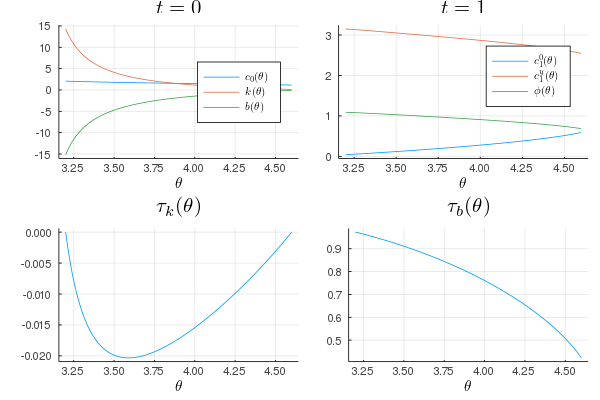
\includegraphics[scale = 0.6]{figures/results_dual.png}
    \label{fig:two_pd}
\end{figure}

These results demonstrate the forces exerted by the moral hazard problem on optimal allocations. Although returns to scale are constant at the individual level, in the aggregate, the model exhibits decreasing returns, as in \cite{shourideh2014optimal}. Specifically, the planner finds it optimal to have a range of \( \theta \)-types invest, rather than just the most productive type. The amount of investment \( k \) allocated to any type is limited by the incentive constraints; in particular, if too much capital is allocated to any one type, then other agents can benefit by reporting this type, eating the entire first-period allocation \( c_0 + k \), and investing and producing nothing. Thus, the role for types of \( \theta<\bar{\theta} \) to become entrepreneurs arises endogenously from the moral hazard problem, rather than from an assumption of decreasing returns to scale.  

\section{Full Dynamic Model} \label{sec:dyn_mod}

While the two-period model of section \ref{sec:two_pd_model} provided a number of insights on optimal taxation in our framework, it does not allow us to differentiate between capital income and wealth. In order to make this distinction, we turn our attention to an infinite horizon model where, with the right assumptions, only slight modifications to the two-period model are needed. 

Time is again discrete and indexed by \( t \). Each period plays out in the following order: an agent begins the period by realizing his capital income \( y_t \), given his prior type \( \theta_{t-1} \) and investment \( k_t \), according to the following process: 
\begin{equation} \label{eqn:dyn_yt}
    y_{t}=\begin{cases}
        \theta_{t-1}k_{t} & \textrm{with probability }\alpha\\
        0 & \textrm{with probability } 1-\alpha
        \end{cases}
\end{equation}
The agent then draws a new type \( \theta_t \) from the same distribution with CDF \( F(\theta) \); these draws are independent and identically distributed across agents and time. Denoting his history of draws \( \theta^t \) and capital incomes \( y^t \), he then makes consumption and savings choices \( c_{t}\left(\theta^{t},y^{t}\right),k_{t+1}\left(\theta^{t},y^{t}\right) \), and \( b_{t+1}\left(\theta^{t},y^{t}\right) \). Let \( \mu_t\left( \theta^t, y^t \right) \) be the measure of period-\( t \) histories induced by the stochastic process governing \( \theta_t \) and the random nature in \( y_t \) described in (\ref{eqn:dyn_yt}). 

The planner chooses allocations \( \left\{ c_{t}\left(\theta^{t},y^{t}\right),k_{t+1}\left(\theta^{t},y^{t}\right),b_{t+1}\left(\theta^{t},y^{t}\right) \right\}_{t=0}^\infty \) in order to solve
\begin{equation}
    \max\sum_{t=0}^{\infty}\beta^{t}\int u\left(c_{t}\left(\theta^{t},y^{t}\right)\right)d\mu_{t}\left(\theta^{t},y^{t}\right) \label{eqn:plan_prob_dyn}
\end{equation}
Subject to a series of feasibility constraints:
\begin{equation}
    \int\left[c_{t}\left(\theta^{t},y^{t}\right)+k_{t+1}\left(\theta^{t},y^{t}\right)\right]d\mu_{t}\left(\theta^{t},y^{t}\right)=\alpha\int\theta_{t-1}k_{t}\left(\theta^{t-1},y^{t-1}\right)d\mu_{t-1}\left(\theta^{t-1},y^{t-1}\right) \label{eqn:rc_dyn}
\end{equation}
As in the static case, the planner's allocations must be incentive compatible. To begin, the promise utility allocated to an agent with history \( \theta^{t} \) conditional on the realization of \( y^{t+1} \) is given by 
\begin{equation}
    w_{t+1}\left(\theta^{t},y^{t+1}\right)=\sum_{s=t+1}^{\infty}\beta^{s-t-1}\int u\left(c_{s}\left(\theta^{s},y^{s}\right)\right)d\mu_{s}\left(\theta^{s},y^{s}|\theta^{t},y^{t+1}\right) \label{eqn:promise_u}
\end{equation}
Thus, upon realization of capital income \( y_{t} \) and report \( \theta^{t} \), the planner allocates consumption and investment to each agent, along with promised utility as given above. Promised utility \( w_t \) is also a sufficient statistic to summarize joint histories \( \left( \theta^t,y^t \right) \), because types \( \theta \) are not autocorrelated. There are two deviation strategies available to the agents. First, they can claim to be type \( \hat{\theta}^{t}\ne\theta^{t} \), and then mimic this type by investing \( \left(\hat{\theta}_{t}/\theta_{t}\right)k\left(\theta^{t-1}, \hat{\theta}^{t}, y^t\right) \). The second available strategy is to claim to be type \( \hat{\theta}_{t} \), eat the entire endowment \( c_{t}+k_{t+1} \), and claim in the next period to have been unlucky. Thus, the allocations must satisfy the following constraints: 
\( \forall\theta^{t},\hat{\theta}_{t},y^{t},t \),
\begin{multline}
    u\left(c_{t}\left(\theta^{t},y^{t}\right)\right)+\beta\left[\alpha w_{t+1}\left(\theta^{t},\left\{ y^{t},y\right\} \right)+\left(1-\alpha\right)w_{t+1}\left(\theta^{t},\left\{ y^{t},0\right\} \right)\right]\geq \\ 
    u\left(c_{t}\left(\theta^{t-1},\hat{\theta}_{t},y^{t}\right)+k\left(\theta^{t-1},\hat{\theta}_{t},y^{t}\right)-\frac{\hat{\theta}_{t}k\left(\theta^{t-1},\hat{\theta}_{t},y^{t}\right)}{\theta_{t}}\right)+ \\ 
    \beta\left[\alpha w_{t+1}\left(\theta^{t-1},\hat{\theta}_{t},\left\{ y^{t},y\right\} \right)+\left(1-\alpha\right)w_{t+1}\left(\theta^{t-1},\hat{\theta}_{t},\left\{ y^{t},0\right\} \right)\right] \label{eqn:ics_t_dyn}
\end{multline}
\begin{multline}
    u\left(c_{t}\left(\theta^{t},y^{t}\right)\right)+\beta\left[\alpha w_{t+1}\left(\theta^{t},\left\{ y^{t},y\right\} \right)+\left(1-\alpha\right)w_{t+1}\left(\theta^{t},\left\{ y^{t},0\right\} \right)\right]\ge \\
    u\left(c_{t}\left(\theta^{t-1},\hat{\theta}_{t},y^{t}\right)+k\left(\theta^{t-1},\hat{\theta}_{t},y^{t}\right)\right)+\beta w_{t+1}\left(\theta^{t-1},\hat{\theta}_{t},\left\{ y^{t},0\right\} \right) \label{eqn:nolie_dyn}
\end{multline}
In formulating these constraints, we rely on the one-shot deviation principle in mechanism design, which allows us to limit our attention to strategies wherein an agent deviates in only one period, rather than multiple periods. Note that the left-hand side of (\ref{eqn:ics_t_dyn}) and (\ref{eqn:nolie_dyn}) both denote the time-\( t \) lifetime utility allocated to an agent of type \( \theta \) who follows the planner's recommendations; we again denote this object \( \mathcal{U}_t\left( \theta^t,y^t \right) \). With this formulation, the problem is a direct analogue of the two-period version. Accordingly, we can employ the same arguments as in section \ref{sec:two_pd_model} in order to simplify the incentive constraints in (\ref{eqn:ics_t_dyn}) and (\ref{eqn:nolie_dyn}). The constraints that we impose, then, are 
\begin{align}
    \frac{\partial}{\partial\theta_{t}}\mathcal{U}\left(\theta^{t},y^{t}\right) &= u^{\prime}\left(c_{t}\left(\theta^{t},y^{t}\right)\right)\frac{k_{t+1}\left(\theta_{t},y^{t}\right)}{\theta_{t}} \label{eqn:ics_local_dyn} \\ 
    \mathcal{U}\left(\underline{\theta}_{t}\right) &\ge u\left(c_{t}\left(\theta^{t},y^{t} \right)+k_{t+1}\left(\theta^{t},y^{t}\right)\right)+\beta w_{t+1}\left(\theta^{t},\left\{ y^{t},0\right\} \right) \label{eqn:nolie_1_dyn}
\end{align}

To solve for allocations in the dynamic setting, we formulate the dual to the planner's problem in (\ref{eqn:plan_prob_dyn}). Here, the planner seeks to minimize the cost of providing a prespecified level of utility \( \mathcal{U}^* \):
\begin{equation}
    \min\sum_{t=0}^{\infty}\frac{1}{\Pi_{s\leq t-1}R_{s}}\int\left[c_{t}\left(\theta^{t},y^{t}\right)-\alpha\theta_{t-1}k_{t}\left(\theta^{t-1},y^{t-1}\right)\right]d\mu_{t}\left(\theta^{t},y^{t}\right) \label{eqn:plan_obj_dual}
\end{equation}
subject to 
\begin{equation}
    \sum_{t=0}^{\infty}\beta^t\int u\left(c_{t}\left(\theta^{t},y^{t}\right)\right)d\mu_{t}\left(\theta^{t},y^{t}\right) \ge \mathcal{U}^* \label{eqn:plan_constr_dual}
\end{equation}
and the incentive constraints in (\ref{eqn:ics_local_dyn}) and (\ref{eqn:nolie_1_dyn}). In order to further simplify the problem, we restrict attention to a component planner, who solves the dual problem for an agent of a particular history \( \left( \theta^t,y^t \right) \) assuming that interest rates are fixed over time. The recursive formulation of the component planner's problem is as follows (suppressing dependence of allocations on current promise utility \( w \)):
\begin{align}
    C\left(w\right)=\min_{c,k',w_{y}^{\prime},w_{0}^{\prime},\mathcal{U}}& \int\left\{ c\left(\theta\right)-\frac{\alpha\theta k\left(\theta\right)}{R}+R^{-1}\left[\alpha C\left(w_{y}^{\prime}\left(\theta\right)\right)+\left(1-\alpha\right)C\left(w_{0}'\left(\theta\right)\right)\right]\right\} dF\left(\theta\right) \label{eqn:plan_rec} \\
    \text{s.t.}& \notag \\
    \int\mathcal{U}\left(\theta\right)dF\left(\theta\right) &\ge w \notag \\
    \mathcal{U}\left(\theta\right) &= u\left(c\right)+\beta\left[\alpha w_{y}^{\prime}\left(\theta\right)+\left(1-\alpha\right)w_{0}^{\prime}\left(\theta\right)\right] \notag \\
    \mathcal{U}^{\prime}\left(\theta\right) &= u^{\prime}\left(c\right)\frac{k}{\theta} \notag \\
    \mathcal{U}\left(\underline{\theta}\right) &\ge u\left(c+k\right)+\beta w_{0}^{\prime} \notag
\end{align}

\subsection{Characterizing Dynamic Allocations} \label{sec:alloc_dyn}

As was the case in the similar model of \cite{shourideh2014optimal}, the value function \( C(w) \) in (\ref{eqn:plan_rec}), along with the attendant policy functions, admit closed-form representations. We assume that utility is given as follows:
\begin{equation}
    u\left(c\right)=\begin{cases}
        \frac{c^{1-\sigma}}{1-\sigma} & \sigma\ne1\\
        \log c & \sigma=1
        \end{cases}
\end{equation}

\begin{proposition} \label{prop:closed_form}
    If \( \sigma = 1 \):
    \begin{align*}
        C(w) &= A\exp\left( \left(1-\beta\right)w \right) &
        w^{\prime}\left(\theta,0,w\right)&=w^{\prime}\left(\theta,0\right)+w \\
        k\left(\theta,w\right)&=k\left(\theta\right)\exp\left(\left(1-\beta\right)w\right) & 
        w^{\prime}\left(\theta,y,w\right)&=w^{\prime}\left(\theta,y\right)+w \\
        c\left(\theta,w\right)&=c\left(\theta\right)\exp\left(\left(1-\beta\right)w\right) &
        \mathcal{U}\left(\theta,w\right)&=\mathcal{U}\left(\theta\right)+w
    \end{align*}
    for some \( A,c\left(\theta\right),k\left(\theta\right),w^{\prime}\left(\theta,y\right),w^{\prime}\left(\theta,0\right) \), and \( \mathcal{U}\left( \theta \right) \). If \( \sigma\ne 1 \), meanwhile, 
    \begin{align*}
        C(w) &= A\left(\left(1-\sigma\right)w\right)^{\frac{1}{1-\sigma}} &
        w^{\prime}\left(\theta,0,w\right)&=w^{\prime}\left(\theta,0\right)\left( 1-\sigma \right)w \\
        k\left(\theta,w\right)&=k\left(\theta\right)\left(\left(1-\sigma\right)w\right)^{\frac{1}{1-\sigma}} & 
        w^{\prime}\left(\theta,y,w\right)&=w^{\prime}\left(\theta,y\right)\left( 1-\sigma \right)w \\
        c\left(\theta,w\right)&=c\left(\theta\right)\left(\left(1-\sigma\right)w\right)^{\frac{1}{1-\sigma}} &
        \mathcal{U}\left(\theta,w\right)&=\mathcal{U}\left(\theta\right)\left( 1-\sigma \right)w
    \end{align*}
\end{proposition}
The proof can be found in the appendix. The key insight is that the planner's problem in (\ref{eqn:plan_rec}) is homogeneous in \( w \). Proposition \ref{prop:closed_form} allows for a much simpler characterization of allocations in the dynamic model than there otherwise may have been. In particular, it gives us the following result:

\begin{proposition} \label{prop:wedge_indep}
    In the dynamic model, the intertemoporal wedges are independent of history \( \left( \theta^t, y^t \right) \). Instead, the wedges \( \tau_{t,k} \) and \( \tau_{t,b} \) depend only on the pair \( \left( \theta_t,\theta_{t+1} \right) \). 
\end{proposition}

The proof is left to the appendix. While proposition \ref{prop:wedge_indep} makes this model much more tractable, it does make the task of implementing the optimal allocations in a decentralized economy somewhat more difficult. Proposition \ref{prop:wedge_indep} states that two individuals with different capital income histories but the same current and next-period types should face the same distortions. As we will demonstrate, however, constructing a tax schedule which induces agents to choose these constrained-efficient allocations will require some care, as it must ensure that two agents of different levels of wealth--but the same type--make identical choices. Note also that a key assumption that led to proposition \ref{prop:wedge_indep} is that the shocks to type \( \theta \) are i.i.d.; while it may seem more natural for entrepreneurial talent to be somewhat persistent, for now, we have not made that the case, in order to gain tractability. 

\subsection{Decentralization} \label{sec:decent}
To this point, we have demonstrated properties of optimal \textit{wedges}, distortions placed on allocations in a mechanism design problem solved by a benevolent social planner. It remains to show how these wedges translate into optimal \textit{taxes} in a dynamic, competitive economy. In order to do so, we consider a decentralized economy, following \cite{benhabib2011distribution}. In this economy, households begin with initial wealth \( w_0 \), and again have the option of intertemporally moving resources by either investing in their own risky entrepreneurial venture, or saving in a risk-free bond. The government observes income from both of these instruments, and levies taxes according to a function \( T \), depending on some combination of capital income \( y \), risk-free interest income \( Rb \), and wealth \( w \). Our goal is to describe the features of the tax function \( T \) that implements the constrained-efficient allocations described in section \ref{sec:alloc_dyn}.

We chose this decentralization in order to most closely match the mechanism design problem that we have studied thus far. Nevertheless, in the mechanism design problem we abstracted away from the nature of private contracts, which we must address in formulating the competitive economy. In particular, in the mechanism design problem we assumed that the agents were able to borrow and lend to one another at risk-free rate \( R \), and that through her allocations, the planner imposed a borrowing constraint and enforced repayment. In the decentralized economy, meanwhile, we must specify how the market for risk-free funds operates, and the degree to which agents can insure themselves against shocks to their type \( \theta \). As a starting point, we make the following assumptions, in order to make the government's role as analogous as possible to that of the planner. 

The market for risk-free funds is operated by an impartial intermediary, who facilitates the sale and purchase of risk-free bonds in whatever amounts the agents choose. Aside from these risk-free savings and transfers from the government, the agents are uninsured from \( \theta \) shocks. The government collects taxes and distributes transfers according to the function \( T \), and in doing so, raises revenue for redistribution, and insures against adverse income shocks (\( y=0 \)). Another choice that must be made in constructing a decentralization is the enforcement of a borrowing constraint, which prevents agents from running Ponzi schemes. Again, we assume that this responsibility falls to the government, which uses the tax function \( T \) to ensure that agents do not choose to borrow more than an exogenous amount \( \ubar{b} \). 

Even given this specification for the decentralization, there are still a number of choices that we must make regarding the tax function. As discussed in section \ref{sec:alloc_dyn}, if we assume that \( \theta \) shocks are i.i.d., we need to choose a tax function that ensures that individuals of the same type, but with different levels of wealth, face the same distortions.

\section{Conclusion} \label{sec:conc}

The prominent role played by capital income risk in generating the thick tail in the distribution of wealth in the US necessitates a better understanding of optimal taxation when agents face risky, heterogeneous returns to investment. To this end, we have presented results on the optimal taxation of capital income in an environment where agents can choose to save in risk-free bonds, or invest capital into an entrepreneurial venture with heterogeneous and uncertain returns. Following prior studies on optimal taxation following \cite{mirrlees1971exploration}, we begin by studying optimal allocations and wedges in a mechanism design problem. We show that in a static two-period model, the optimal tax on risky capital is U-shaped and negative, with a marginal tax of zero on the least and most productive entrepreneurs and a subsidy to everyone else. The optimal tax on risk-free interest, meanwhile, is positive for entrepreneurs, steering them away from savings and towards productive--but risky--investment. In the dynamic model, meanwhile, we demonstrate that optimal intertemoporal wedges are independent of history, and instead depend only on current and next-period type. 

We then turn to a decentralized economy, in which agents can borrow and lend at the risk-free rate in a sequence of spot markets, and the government uses taxes and transfers to provide    partial insurance to entrepreneurs and enforce a limit on borrowing. Our next step in this exercise is to construct a tax function that implements the constrained-efficient allocations in the decentralized economy. In addition, we plan to examine how the nature of allocations in the dynamic model changes when \( \theta_t \) exhibits persistence over time. 

\bibliographystyle{named}
\bibliography{summer_paper}
\newpage
\section*{Appendix}
\setcounter{equation}{0}
\renewcommand{\theequation}{A.\arabic{equation}}

In the arguments that follow, we suppress the dependence of the allocations on \( \theta \); for instance, we substitute \( c_0 = c_0(\theta) \) and \( c_1^y = c_1\left( \theta,y \right) \).

\paragraph{First-Order Approach} 
An equivalent formulation of the incentive constraints in (\ref{eqn:ics}) is:
\begin{equation}
    \mathcal{U}\left(\theta\right)=\max_{\hat{\theta}}u\left(c_{0}\left(\hat{\theta}\right)\right)+\beta\left(\alpha u\left(\theta k\left(\hat{\theta}\right)+Rb\left(\hat{\theta}\right)-T\right)+\left(1-\alpha\right)u\left(Rb-T\right)\right)
\end{equation}
The envelope condition gives
\begin{equation}
    \mathcal{U}^{\prime}\left(\theta\right)=\beta\alpha\left(1-T_{1}\right)ku^{\prime}\left(c_{1}^{y}\right) \label{eqn:foa_env}
\end{equation}
The household optimality condition for \( k \), meanwhile, gives 
\begin{equation}
    u^{\prime}\left(c_{0}\right)=\beta\alpha\theta\left(1-T_{1}\right)u^{\prime}\left(c_{1}^{y}\right) \label{eqn:foa_eul}
\end{equation}
Combining (\ref{eqn:foa_env}) and (\ref{eqn:foa_eul}) gives 
\begin{equation*}
    \mathcal{U}^\p\left( \theta \right) = u^\p(c_0)\frac{k}{\theta}
\end{equation*}
the form in (\ref{eqn:ic_t}).

\paragraph{Proof of Proposition \ref{prop:cutoff}}
\begin{proof}
    The proof proceeds by contradiction. Assume that for some $\theta$,
$k\left(\theta\right)>0$ at the optimum of the planner's problem,
but $\alpha\theta<R$. Then, from the first-order condition for $k$
in the planner's problem, 
\[
R-\alpha\theta=\frac{\mu}{\lambda_{1}\theta c_{0}}-\frac{\phi}{\lambda_{1}\left(c_{0}+k\right)}>0
\]
which implies that 
\[
\frac{\mu}{\lambda_{1}\theta c_{0}}>\frac{\phi}{\lambda_{1}\left(c_{0}+k\right)}>0
\]
Thus, $\mu$--the multiplier on the incentive constraint--is positive.
Then, rearranging the first-order conditions for $c_{0}$ and $k$
gives
\begin{align*}
R+\frac{\phi}{\lambda_{1}\left(c_{0}+k\right)}= & \frac{c_{1}^{y}}{\beta c_{0}}-\frac{\mu k}{\lambda_{1}\theta c_{0}^{2}}\\
R+\frac{\phi}{\lambda_{1}\left(c_{0}+k\right)}= & \alpha\theta+\frac{\mu}{\lambda_{1}\theta c_{0}}
\end{align*}
which implies
\[
R+\frac{\phi}{\lambda_{1}\left(c_{0}+k\right)}=\frac{c_{1}^{y}}{\beta c_{0}}-\frac{k}{c_{0}}\left(\underbrace{R+\frac{\phi}{\lambda_{1}\left(c_{0}+k\right)}-\alpha\theta}_{>0}\right)
\]
The term in parentheses on the right-hand side is equal to $\frac{\mu}{\lambda_{1}\theta c_{0}}$,
which by the above, is positive. This implies that 
\[
\frac{c_{1}^{y}}{\beta c_{0}}>R+\frac{\phi}{\lambda_{1}\left(c_{0}+k\right)}
\]
This, however, implies that $\mu<0$, contradicting the assumption.
Thus, $k\left(\theta\right)>0\implies\alpha\theta>R$.

The first-order condition for $c_{1}\left(\theta,0\right)$, meanwhile,
can be rearranged to give 
\begin{equation}
    c_{1}^{y}=c_{1}^{0}+\frac{\beta\phi}{\lambda_{1}\left(1-\alpha\right)} \label{eqn:incentive_proof}
\end{equation}
By definition, $\phi\ge0$, with equality if the constraint in (\ref{eqn:nolie1})
does not hold. Equation (\ref{eqn:incentive_proof}) shows that $k>0\implies\phi>0$;
otherwise, the agents would have no incentive to bear the risk of
investing. 
\end{proof}
\paragraph{Proof of Proposition \ref{prop:wedges}}
\begin{proof}
    Recall that the intertemporal wedges are given by 
\begin{align*}
\tau_{k}\left(\theta\right)= & 1-\frac{c_{1}^{y}}{\alpha\beta\theta c_{0}}\\
\tau_{b}\left(\theta\right)= & 1-\frac{\frac{1}{c_{0}}}{\beta R\left(\frac{\alpha}{c_{1}^{y}}+\frac{1-\alpha}{c_{1}^{0}}\right)}
\end{align*}
Begin with the case where $k>0$. Combining the first-order conditions
in the planner's problem for $c_{0}$ and $k$ gives 
\[
\frac{c_{1}^{y}}{\beta c_{0}}-\frac{\mu k}{\lambda_{1}\theta c_{0}^{2}}=\alpha\theta+\frac{\mu}{\lambda_{1}\theta c_{0}}
\]
which implies
\begin{align*}
\alpha\theta-\frac{c_{1}^{y}}{\beta c_{0}} & =\frac{\mu}{\lambda_{1}\theta c_{0}}\left(-\frac{k}{c_{0}}-1\right)\\
\tau_{k}=1-\frac{c_{1}^{y}}{\alpha\beta\theta c_{0}} & =\frac{\mu}{\lambda_{1}\alpha\theta^{2}c_{0}}\left(-\frac{k}{c_{0}}-1\right)
\end{align*}
In practice, \( \mu\ge 0 \), and so because all other variables on the right-hand side of the final equality are nonnegative, the above shows that $\tau_{k}\le0$. The boundary conditions in the planner's problem are \( \mu\left( \ubar{\theta} \right) = \mu\left( \bar{\theta} \right) = 0 \), and thus \( \tau_k\left( \ubar{\theta} \right) = \tau_k\left( \bar{\theta} \right) = 0 \) by the above. 

Turning to the
wedge on risk-free savings, note that if $k\left(\theta\right)>0$,
then period-1 consumption $c_{1}\left(\theta\right)$ becomes a random
variable, so by Jensen's inequality, 
\begin{align*}
\frac{\alpha}{c_{1}^{y}}+\frac{1-\alpha}{c_{1}^{0}} & >\frac{1}{\alpha c_{1}^{y}+\left(1-\alpha\right)c_{1}^{0}}\implies\\
\alpha c_{1}^{y}+\left(1-\alpha\right)c_{1}^{0} & >\frac{1}{\frac{\alpha}{c_{1}^{y}}+\frac{1-\alpha}{c_{1}^{0}}}\implies\\
\frac{\alpha c_{1}^{y}+\left(1-\alpha\right)c_{1}^{0}}{\beta Rc_{0}} & >\frac{\frac{1}{c_{0}}}{\beta R\left(\frac{\alpha}{c_{1}^{y}}+\frac{1-\alpha}{c_{1}^{0}}\right)}
\end{align*}
So in order to establish a positive wedge $\tau_{b}$, it is sufficient
to show that $\beta Rc_{0}>\alpha c_{1}^{y}+\left(1-\alpha\right)c_{1}^{0}$.
From the first-order conditions in the planner's problem, 
\begin{align*}
\alpha c_{1}^{y}+\left(1-\alpha\right)c_{1}^{0} & =c_{1}^{y}-\frac{\beta\phi}{\lambda_{1}}
\end{align*}
and
\[
\beta Rc_{0}=c_{1}^{y}-\frac{\beta\mu k}{\lambda_{1}\theta c_{0}}-\frac{\beta\phi c_{0}}{\lambda_{1}\left(c_{0}+k\right)}
\]
Combining and multiplying through by $\left(-\beta/\lambda_{1}\right)$,
it suffices to show that 
\[
\phi\left(1-\frac{c_{0}}{c_{0}+k}\right)\ge\frac{\mu k}{\theta c_{0}}
\]
Note, however, that this inequality holds trivially when \( k\left( \theta \right) >0 \): by definition,
the left hand side is positive, while the right is negative.

In the case where $k\left(\theta\right)=0$, $c_{1}\left(\theta,y\right)=c_{1}\left(\theta,0\right)\equiv c_{1}\left(\theta\right)$;
the planner does not find it optimal for these types to invest, and
so she has no need to incentivize them to do so. By Proposition \ref{prop:cutoff},
then, $\phi\left(\theta\right)=0$. Then, the first-order condition
for $c_{0}\left(\theta\right)$ in the planner's problem gives
\[
1=\frac{c_{1}}{\beta Rc_{0}}
\]
and thus $\tau_{b}\left(\theta\right)=0$ for types who do not invest. 
\end{proof}

\paragraph{Proof of Proposition \ref{prop:closed_form}}
\begin{proof}
    
    Begin with the case where \( \sigma = 1 \). Under the posited form for the value and policy functions, the component planner's problem becomes
    
    \begin{multline}
        A=\min\\\int\left\{ c\left(\theta\right)+k\left(\theta\right)-\frac{\alpha\theta k\left(\theta\right)}{R}+\frac{1}{R}\left[\alpha A\exp\left(\left(1-\beta\right)w_{y}^{\prime}\left(\theta\right)\right)+\left(1-\alpha\right)A\exp\left(\left(1-\beta\right)w_{0}^{\prime}\left(\theta\right)\right)\right]\right\} dF\left(\theta\right) \label{eqn:vf_log}
    \end{multline}
    Subject to 
    \begin{align*}
        0&=\int\mathcal{U}\left(\theta\right)dF\left(\theta\right)\\
        \mathcal{U}\left(\theta\right)&=\log c\left(\theta\right)+ \beta\left[\alpha w_{1}'\left(\theta\right)+\left(1-\alpha\right)w'_{0}\left(\theta\right)\right]\\
        \mathcal{U}^{\prime}\left(\theta\right)&=\frac{k\left(\theta\right)}{\theta c\left(\theta\right)}\\
        \mathcal{U}\left(\underline{\theta}\right)&=\log\left(c\left(\theta\right)+k\left(\theta\right)\right)+\beta w'_{0}\left(\theta\right)
    \end{align*}
    Note that now the problem is independent of \( w \). Thus, the existence of \( A \) as the solution to the problem in (\ref{eqn:vf_log}) proves the proposition. We use Blackwell's sufficient conditions to verify that the mapping on the right-hand side of (\ref{eqn:vf_log}), denoted \( (TA)(w) \), is a contraction mapping, with a fixed point of \( A \). First, this mapping satisfies monotonicity: consider two sets of policy functions \( \{c(\theta), k(\theta), w_y^\p(\theta), w_0^\p(\theta), \mathcal{U}(\theta)\} \), one uniformly higher than the other. Clearly, the total cost of delivering utility under the greater of the policy functions will have a higher cost, and thus this mapping is monotonic. In addition, 
    \begin{align*}
        &T\left(A+a\right)\left(w\right)=\text{\ensuremath{\min}} \\ &\int\left[c\left(\theta\right)+k\left(\theta\right)-\frac{\alpha\theta k\left(\theta\right)}{R}+\frac{1}{R}\alpha\left\{ A\exp\left(\left(1-\beta\right)w_{y}^{\prime}\left(\theta\right)\right)+a\right\} +\frac{1}{R}\left(1-\alpha\right)\left\{ A\exp\left(\left(1-\beta\right)w_{y}^{\prime}\left(\theta\right)\right)+a\right\} \right]\\
        &=T\left(A\right)+a\frac{1}{R}
    \end{align*}
    As long as \( R>1 \), this mapping is a contraction, and has a fixed point \( A(w) \). However, since the problem was independent of \( w \), \( A(w) \) is a constant \( A \). 

    The case where \( \sigma\ne 1 \) is similarly shown. Under the posited forms, when \( w = \left( 1-\sigma \right)^{-1} \), the planner solves 
    \begin{align}
        A&=\text{\ensuremath{\min}} \notag \\
        \int&\left\{ c\left(\theta\right)+k\left(\theta\right)-\frac{\alpha\theta k\left(\theta\right)}{R}+\frac{1}{R}\left[\alpha A\left(\left(1-\sigma\right)w_{y}^{\prime}\right)^{\frac{1}{1-\sigma}}+\left(1-\alpha\right)A\left(\left(1-\sigma\right)w_{0}^{\prime}\right)^{\frac{1}{1-\sigma}}\right]\right\} dF\left(\theta\right) \label{eqn:vf_ces}
    \end{align}
    By the same arguments as in the case where \( \sigma = 1 \), \( A \) exists as the fixed point of the contraction map defined by the right-hand side of (\ref{eqn:vf_ces}). 
\end{proof}

\paragraph{Proof of Proposition \ref{prop:wedge_indep}}
\begin{proof}
In the dynamic model, the intertemporal wedge on risky capital is given by 
\begin{equation}
    \tau_{t,k}\left(\theta^{t},y^{t}\right)=1-\frac{u^{\prime}\left(c_{t}\left(\theta^{t-1},y^{t}\right)\right)}{\alpha\beta\theta_{t}u^{\prime}\left(c_{t+1}\left(\theta^{t+1},\left\{ y^{t},y\right\} \right)\right)} \label{eqn:app_dyn_tauk}
\end{equation}
Consider the case \( \sigma = 1 \). Under proposition \ref{prop:closed_form}, 
\begin{align*}
    c_{t}\left(\theta^{t},y^{t}\right)&=c\left(\theta_{t}\right)\exp\left(\left(1-\beta\right)w_{t}\left(\theta^{t-1},y^{t}\right)\right)\\
    w_{t+1}\left(\theta^{t},\left\{ y^{t},y\right\} \right)&=w_{t}\left(\theta^{t-1},y^{t}\right)+w_{t+1}^{y}\left(\theta_{t}\right)
\end{align*}
and furthermore,
\begin{align*}
    c_{t+1}\left(\theta^{t+1},\left\{ y^{t},y\right\} \right)&=c\left(\theta_{t+1}\right)\exp\left[\left(1-\beta\right)w_{t+1}\left(\theta^{t},\left\{ y^{t},y\right\} \right)\right]\\
    &=c\left(\theta_{t+1}\right)\exp\left[\left(1-\beta\right)\left\{ w_{t}\left(\theta^{t-1},y^{t}\right)+w_{t+1}^{y}\left(\theta_{t}\right)\right\} \right]
\end{align*}
Thus, the wedge in (\ref{eqn:app_dyn_tauk}) can be written as 
\begin{align*}
    \tau_{t,k}\left(\theta^{t},y^{t}\right)&=1-\frac{1/c_{t}\left(\theta^{t},y^{t}\right)}{\alpha\beta\theta_{t}\left\{ 1/c_{t+1}\left(\theta^{t+1},\left\{ y^{t},y\right\} \right)\right\} }\\
    &=1-\frac{1/c\left(\theta_{t}\right)\exp\left(\left(1-\beta\right)w_{t}\left(\theta^{t-1},y^{t}\right)\right)}{\alpha\beta\theta_{t}\left\{ 1/c\left(\theta_{t+1}\right)\exp\left[\left(1-\beta\right)\left\{ w_{t}\left(\theta^{t-1},y^{t}\right)+w_{t+1}^{y}\left(\theta_{t}\right)\right\} \right]\right\} }\\
    &=1-\frac{1/c\left(\theta_{t}\right)\exp\left(\left(1-\beta\right)w_{t}\left(\theta^{t-1},y^{t}\right)\right)}{\alpha\beta\theta_{t}\left\{ 1/c\left(\theta_{t+1}\right)\exp\left[\left(1-\beta\right)w_{t}\left(\theta^{t-1},y^{t}\right)\right]\exp\left[\left(1-\beta\right)w_{t+1}^{y}\left(\theta_{t}\right)\right]\right\} }\\
    &=1-\frac{1/c\left(\theta_{t}\right)}{\alpha\beta\theta_{t}\left\{ 1/c\left(\theta_{t+1}\right)\exp\left[\left(1-\beta\right)w_{t+1}^{y}\left(\theta_{t}\right)\right]\right\} }
\end{align*}
The final line gives the desired result: \( \tau_{t,k}\left(\theta^{t},y^{t}\right) \) only depends on \( \theta_t \) and \( \theta_{t+1} \). The wedge on risk-free savings is similar:
\begin{align*}
    \tau_{t,b}\left(\theta^{t},y^{t}\right)&=1-\frac{1/c_{t}\left(\theta^{t},y^{t}\right)}{\beta R\left[\alpha/c_{t+1}\left(\theta^{t+1},\left\{ y^{t},y\right\} \right)+\left(1-\alpha\right)/c_{t+1}\left(\theta^{t+1},\left\{ y^{t},0\right\} \right)\right]}\\
    &=1-\frac{1/c\left(\theta_{t}\right)}{\beta R\left\{ \alpha/c\left(\theta_{t+1}\right)\exp\left[\left(1-\beta\right)w_{t+1}^{y}\left(\theta_{t}\right)\right]+\left(1-\alpha\right)/c\left(\theta_{t+1}\right)\exp\left[\left(1-\beta\right)w_{t+1}^{0}\left(\theta_{t}\right)\right]\right\} }
\end{align*}
Thus, \( \tau_{t,b} \) also depends only on \( \theta_t \) and \( \theta_{t+1} \). The same can easily be shown for the case where \( \sigma \ne 1 \). 
\end{proof}

\end{document}